\chapter{Project Design}

Chapter 3 defines the system requirements and lays out the methodology, the design decisions, and the project plan with the task allocation. The first section records the functional and nonfunctional requirements together with the context diagram, the level-one data flow diagram, and the interface design.

\section{Requirement Analysis}\label{sec:requirement-analysis}

Requirement analysis fixes what the framework must do before any code is written. The system is an experimental deliberation layer rather than a conventional application, so the requirements are framed around the research pipeline. A question enters, agents debate it over a fixed number of rounds, the claims are checked against external evidence, and a trust-weighted answer comes out. A multi-agent debate approach is used here since prior research indicates it yields more factual responses than relying on a single model ~\cite{du2024improving}. Furthermore, we incorporated a trust mechanism to prevent situations where a confident but incorrect majority forces a correct minority agent to change its answer ~\cite{pitre-etal-2025-consensagent}. The below sections will provide detail on the individual components of the System Requirements for this project including Boundaries, Data Flows and the User Interface for the Framework.
\subsection{Functional and Nonfunctional Requirements}\label{subsec:requirements}

The Functional Requirements outline the primary functions that the framework provides. All input questions (from both the User and/or the Evaluation Harness) are processed in complete ignorance of their actual "ground-truth" as it relates to the Agents. In order to be efficient, all input questions do not require a full debate. Therefore, an initial Confidence Gate determines whether an input question should receive a Direct Response or be sent to the Main Pipeline for processing. The Orchestration Process controls 3 different Heterogeneous LLM Agents, each revising at most 3 times per Agent (via State Machine), as determined by 3 retry limits.

Each Agent's Reasoning is segmented into Atomic Factual Claims and carefully tagged to its Source. If this structured tagging process fails, a fallback extraction pass is triggered to handle the unparsed text. Retrieval gives each agent its own database: PubMed for the first, arXiv for the second, Semantic Scholar for the third. OpenAlex stands in when a source is down, and a cross-encoder reranks the passages that come back. Each claim then lands on one of four verdicts: supported, contradicted, unverifiable, or contested.

After every round the trust score is updated as $S_i(t+1) = S_i(t) + \alpha V_i - \beta H_i$. A softmax follows, the values are clamped between 0.1 and 0.9, and the vector is renormalized.

Those two bounds matter. Without them an agent could be silenced outright, or could grow to dominate the debate. An injection point lets the harness insert a fabricated wrong consensus between rounds. That is how sycophantic collapse gets measured under controlled pressure. At the end, weighted aggregation over trust and position picks the final answer, and the majority vote plays no part in it. The results package contains
the answers, the citations supporting those answers, the full trust history, and the reasoning trace for each agent..

The evaluation harness will compute an estimate of the answer's correctness along with a measure of how well the framework has collapsed into a consensus, preserved minority opinions, and calibrated its use of evidence. It will evaluate
this framework relative to baseline methods based upon majority voting and MoA~\cite{wang2025mixture}, iMAD~\cite{fan2026imad}, and DebUnc~\cite{yoffe-etal-2025-debunc} .There are several built-in recovery routes in case there is some kind of failure within the system. For example, if a model's output cannot be processed then it will be sent through the fallback extraction path. Any timeouts encountered during this process will be retried one time prior to the current round being declared as inconclusive. Additionally, if a retrieval API becomes unavailable then the system will either default to using available cached evidence or make queries directly to OpenAlex.

With respect to non-functional requirements, which refer to properties of systems, such as performance and scalability, but do not describe specific behavior, latency is currently the most significant limiting factor. This is achieved by forcing adherence to the limit of three debate rounds plus three retries. This ensures that total processing times remain reasonable on the intended hardware. The system was also designed such that when a single component fails, it does not bring down the entire debate. Instead, failure is dealt with at a local level while keeping other components active. Portability is another important design consideration. By utilizing the vLLM interface compatible with OpenAI, the framework supports both closed APIs and locally hosted models with equal ease. For practical purposes, the same pipeline can operate unmodified on both our development models (Qwen3.5-9B, Gemma 4 12B, Ministral-3-14B), as well as the final evaluation models (Qwen3.6-27B, Gemma 4 26B, Mistral Small 3.2 24B). No fine tuning is required for inference, nor is it computationally intensive, allowing it to run on a single rented GPU from NVIDIA - specifically an RTX PRO 6000 Blackwell 96GB. Using this GPU costs approximately USD 0.70 to 1.90 per hour. Finally, to facilitate transparency and reproducibility all runs are seeded appropriately and all relevant intermediate outputs are logged. This allows the final output to maintain an auditable decision trail detailing which agent's claims were supported or contradicted by the evidence. Throughout this process, the ground truth remains completely hidden from the agents, and the final provided answer explicitly cites its supporting evidence.

\subsection{Context Diagram}\label{subsec:context-diagram}

As illustrated in Figure ~\ref{fig:context-diagram}, the context diagram outlines the system boundaries and identifies the external actors interacting with the framework. The core system is positioned at the center, receiving input questions either directly from a user or via the evaluation harness. Scientific passages come back from three external databases, and off-the-shelf language models are called through the vLLM server on a rented RTX PRO 6000 Blackwell GPU. The evaluation harness receives the scores, and the user gets the final result package with the answer, the citations, the trust trajectory, and each reasoning trace.

\begin{figure}[ht]
  \centering
  \resizebox{\textwidth}{!}{%
    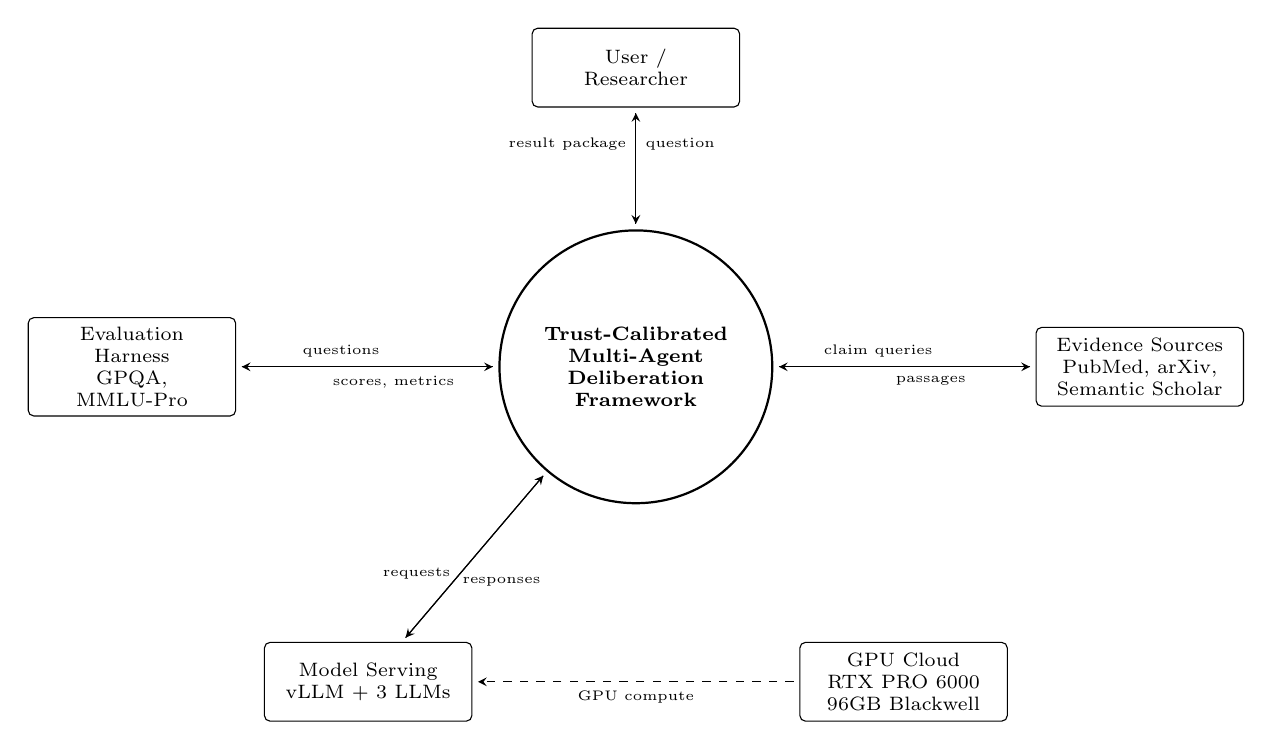
\begin{tikzpicture}[
        entity/.style={draw, rounded corners=2pt, text width=2.4cm, align=center, minimum height=1.0cm, font=\scriptsize},
        sysbox/.style={draw, thick, circle, text width=3.0cm, align=center, font=\scriptsize\bfseries},
        flow/.style={->, >=stealth, shorten >=2pt, shorten <=2pt, font=\tiny}
      ]
      \node[sysbox] (sys) at (0,0) {Trust-Calibrated\\Multi-Agent\\Deliberation\\Framework};
      \node[entity] (user) at (0,3.8) {User /\\Researcher};
      \node[entity] (eval) at (-6.4,0) {Evaluation\\Harness\\GPQA, MMLU-Pro};
      \node[entity] (src) at (6.4,0) {Evidence Sources\\PubMed, arXiv,\\Semantic Scholar};
      \node[entity] (models) at (-3.4,-4.0) {Model Serving\\vLLM + 3 LLMs};
      \node[entity] (gpu) at (3.4,-4.0) {GPU Cloud\\RTX PRO 6000\\96GB Blackwell};

      \draw[flow] (user) -- node[right, pos=0.3] {question} (sys);
      \draw[flow] (sys) -- node[left, pos=0.7] {result package} (user);
      \draw[flow] (eval) -- node[above, pos=0.4] {questions} (sys);
      \draw[flow] (sys) -- node[below, pos=0.4] {scores, metrics} (eval);
      \draw[flow] (sys) -- node[above, pos=0.4] {claim queries} (src);
      \draw[flow] (src) -- node[below, pos=0.4] {passages} (sys);
      \draw[flow] (sys) -- node[left, pos=0.6] {requests} (models);
      \draw[flow] (models) -- node[right, pos=0.35] {responses} (sys);
      \draw[flow,dashed] (gpu) -- node[below, pos=0.5] {GPU compute} (models);
    \end{tikzpicture}}
  \caption{Context diagram of the trust-calibrated multi-agent deliberation framework.}
  \label{fig:context-diagram}
\end{figure}

\subsection{Data Flow Diagram Level 1}\label{subsec:dfd-level1}

The level-one data flow diagram in Figure~\ref{fig:dfd-level1} decomposes the framework into seven processes. A question enters through the intake and gate process, which decides between a direct answer and a debate. Orchestration runs the revision rounds. It sends inference requests to the external models and reads and writes the debate state. Each position is decomposed into atomic claims and verified against the external sources. The verdicts then drive the trust update, which writes the new trust values back into the debate state. At the last round, weighted aggregation selects the answer and the packaging process logs the result before it returns to the user. Three data stores hold the debate state, the evidence and verdict log, and the results log.

The diagram reads from left to right and top to bottom. The evaluation harness submits a question, and the confidence gate decides whether the debate is worth running. The orchestration process then asks the model server for the agent positions. Positions are decomposed into atomic claims, and the retrieval process verifies them against the external sources. The verdicts are stored in the evidence log before they drive the trust update. The updated trust is written back into the debate state, so the next round starts from the corrected influence values. At the last round the aggregation process selects the answer. The packaging process logs it in the results log, and the result package with the answer and the citations returns to the user.

\begin{figure}[ht]
  \centering
  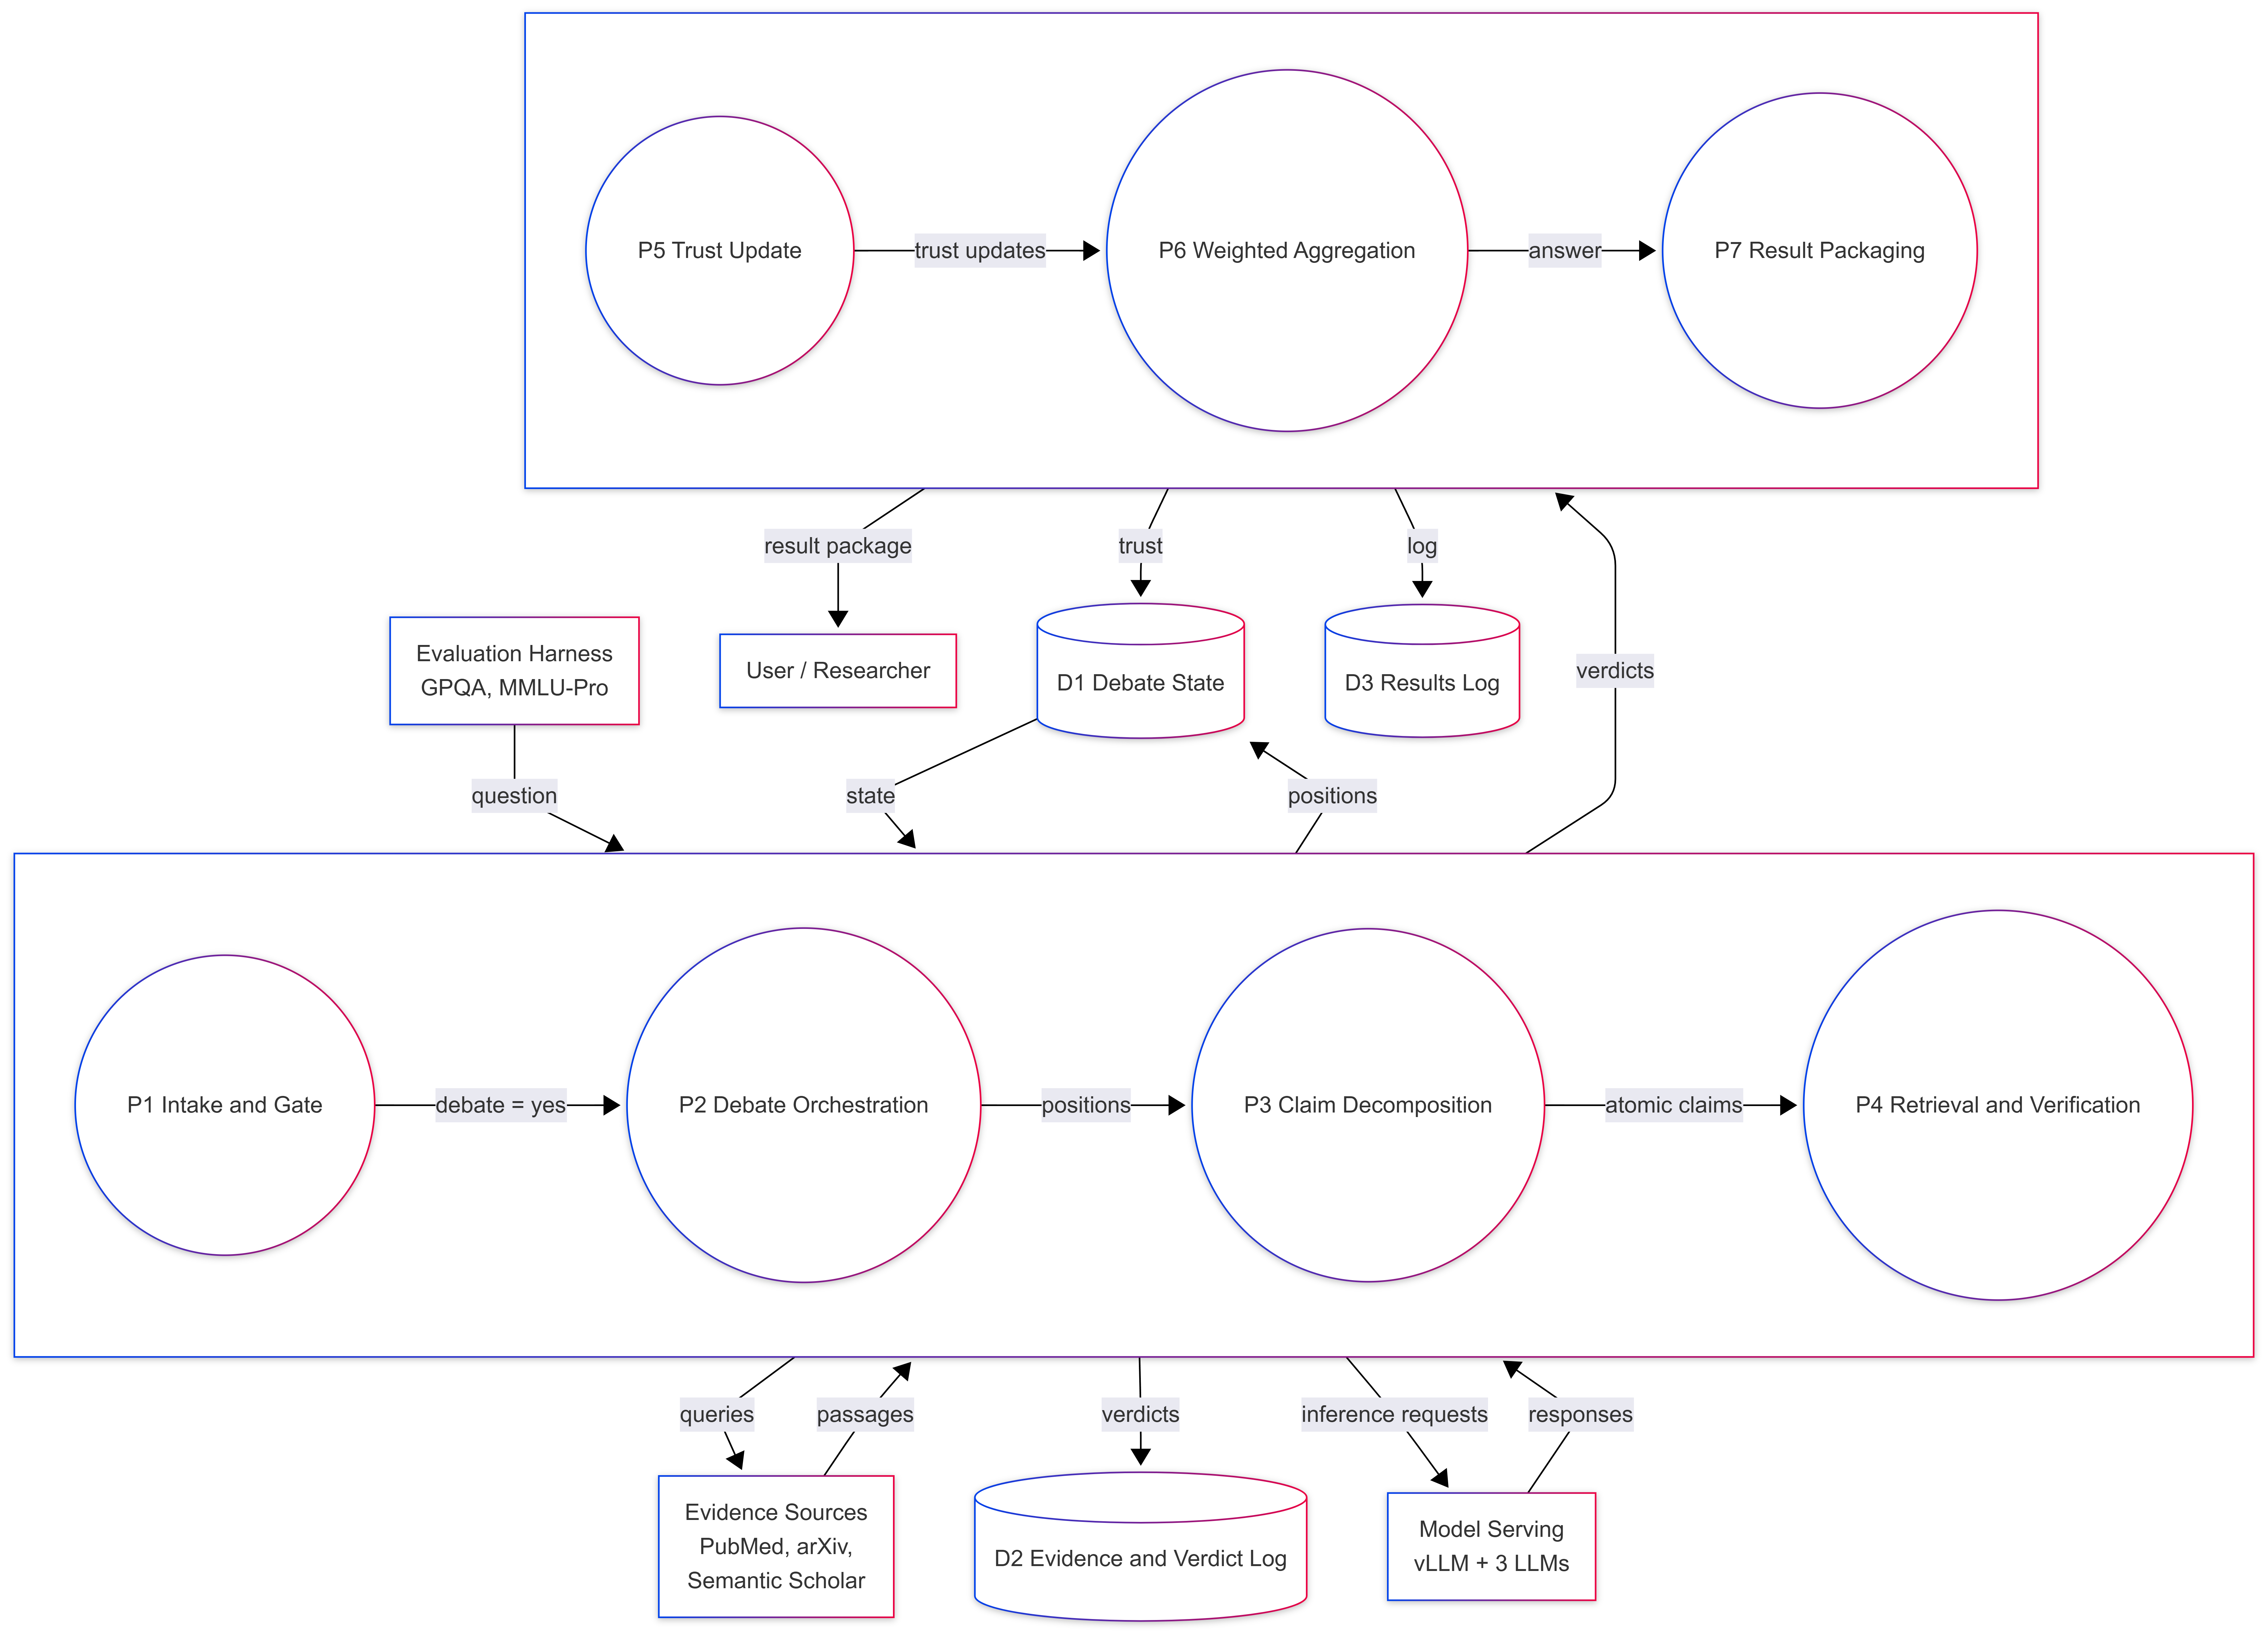
\includegraphics[width=\textwidth]{data-flow.png}
  \caption{Level-one data flow diagram of the trust-calibrated multi-agent deliberation framework.}
  \label{fig:dfd-level1}
\end{figure}

\subsection{UI Design}\label{subsec:ui-design}

The framework is operated through a command-line interface and a small web dashboard. The command-line interface starts experiments and points the pipeline at the evaluation datasets. Every run is written to a JSON package. It is the primary interface because the system runs in batches on a rented GPU, where a graphical interface adds little value. The web dashboard is used afterwards to inspect single debates. It shows the agents as cards with their current positions, plus a chart of the trust trajectory across rounds and the verdict of every claim with the passage that supports or contradicts it. This is where the transparency of the framework becomes visible, because a user can trace exactly why an agent lost influence. Figure~\ref{fig:cli} and Figure~\ref{fig:dashboard} show the intended layout of both interfaces. The screenshots will be replaced with the real output of the system once the implementation is complete.

\begin{figure}[ht]
  \centering
  \fbox{\parbox[c][6cm][c]{0.8\textwidth}{\centering Screenshot of the command-line experiment interface.}}
  \caption{Command-line interface for running experiments and writing JSON result packages.}
  \label{fig:cli}
\end{figure}

\begin{figure}[ht]
  \centering
  \fbox{\parbox[c][6cm][c]{0.8\textwidth}{\centering Screenshot of the debate inspection dashboard.}}
  \caption{Web dashboard showing agent positions, the trust trajectory, and per-claim evidence verdicts.}
  \label{fig:dashboard}
\end{figure}

\section{Detailed Methodology and Design}

\section{Project Plan}\label{sec:project-plan}

The project runs for ten months, from Month 1 to Month 10, and covers 40 weeks.
It is split into eight phases with six review gates. The work starts with literature
and setup and ends with writing and submission. Table~\ref{tab:phases} lists each
phase with its weeks and deliverables. Table~\ref{tab:gates} lists the gates and
their checkpoints. Table~\ref{tab:swot} adds a SWOT view of the plan. This report
covers work through the mid-project review in Month 5, while later phases carry
the project to the final defence.

The plan starts with scoping. Project scoping in Phase-0 fixes the research question, the trust-calibrated idea, the evaluation shape, and the gate criteria. Data and model work runs in parallel. Datasets GPQA and MMLU-Pro are checked, and the three development models are chosen with their serving setup. Analysis of the baseline follows in Phase-1. Injection tests and baselines B1 to B4 are run, and the pilot checks if a wrong majority can still fool voting. Design and implement fill Phase-2. Claim decompositions and source partitioned RAG are created. Additionally, the trust function is adjusted by setting its clamp and softmax. In addition to this, a short dry-run and a design freeze marks the end of Phase-2 to 3. Phase-3a holds the main studies which were implemented under Phase-3a's core conditions using three seed implementations. Phase-3b contains ablation studies implementing different agent numbers as well as different alpha/beta combinations. The human study (and failure reviews) occur in Phase-4. Finally, writing, reproducibility packaging, submission, and defense preparations complete the project in Phase-5.

\begin{center}
  \begin{table}[ht]
    \centering
    \caption{Project phases with week-level durations and deliverables.}
    \renewcommand{\arraystretch}{1.6}
    \begin{tabular}{|p{0.22\textwidth}|p{0.16\textwidth}|p{0.50\textwidth}|}
      \hline
      Phase                                  & Duration                 & Deliverables                                                                                        \\
      \hline
      Phase-0: Literature and Setup          & Month 1 (Wk 1--4)        & Literature freeze, vLLM and LangGraph setup, model identification, vanilla MAD reproduction         \\
      Phase-1: Injection and Baselines       & Month 2 (Wk 5--8)        & Injection protocol, baselines B1--B4, Proposition 1 proof, month-end pilot                          \\
      Phase-2: Trust Mechanism Build         & Months 3--4 (Wk 9--16)   & Claim decomposition, source-partitioned RAG, trust function v1, baselines B5/B6/B9                  \\
      Phase-2 to 3: Mid-Project              & Month 5 (Wk 17--20)      & Design freeze, dry run on one dataset, FYDP-1 defence preparation, and review feedback fixes        \\
      Phase-3a: Main Experiments             & Month 6 (Wk 21--24)      & Core conditions on primary datasets, three seeds, 95\% confidence intervals, and effect size report \\
      Phase-3b: Ablations and Scaling        & Month 7 (Wk 25--28)      & Four ablations, $\alpha$/$\beta$ sweep, $N \in \{2,3,5\}$, and results freeze                       \\
      Phase-4: Human Evaluation and Analysis & Month 8 (Wk 29--32)      & Human evaluation with $n=60$, ECR calibration, failure analysis, and buffer for slippage            \\
      Phase-5: Writing and Submission        & Months 9--10 (Wk 33--40) & Thesis and paper drafting, reproducibility package, submission, and FYDP-2 defence preparation      \\
      \hline
    \end{tabular}
    \label{tab:phases}
  \end{table}
\end{center}

\begin{center}
  \begin{table}[ht]
    \centering
    \caption{Review gates and their checkpoints.}
    \renewcommand{\arraystretch}{1.6}
    \begin{tabular}{|p{0.26\textwidth}|p{0.18\textwidth}|p{0.42\textwidth}|}
      \hline
      Gate              & Due            & Checkpoint                                                                                              \\
      \hline
      Gate 0            & End of Month 1 & Vanilla MAD reproduces the Du et al. baseline on a GPQA slice, and the reference list is frozen         \\
      Gate 1 (Go/No-Go) & End of Month 2 & Injection validation reaches $\kappa \geq 0.75$, baseline CCR sits at 0.30 or higher, pilot executed    \\
      Gate 2            & End of Month 4 & Trust mechanism plus source-partitioned RAG plus competitor baselines, first CCR and MPR on one dataset \\
      FYDP-1 Defence    & Month 5        & Mid-project report with design freeze and initial results                                               \\
      Gate 3            & End of Month 7 & Full results freeze with confidence intervals and effect sizes                                          \\
      Submit and FYDP-2 & Months 9--10   & Paper submitted, thesis completed, final defence                                                        \\
      \hline
    \end{tabular}
    \label{tab:gates}
  \end{table}
\end{center}

\begin{center}
  \begin{table}[ht]
    \centering
    \caption{SWOT analysis for the project plan.}
    \renewcommand{\arraystretch}{1.6}
    \begin{tabular}{|p{0.44\textwidth}|p{0.44\textwidth}|}
      \hline
      \textbf{Strengths}                                                                                                                                                                                                                & \textbf{Weaknesses} \\
      \hline
      Clear gap on sycophantic consensus, bounded trust design with no fine-tuning, six-member team with mixed skills, and expert supervision that keeps scope tight. The design needs no new training and runs on a single rented GPU. &
      Sparse retrieval on rare claims, imperfect claim split, correlated reasoning errors between agents, and limited GPU budget for 300 hours. Small sample noise in early pilots can also hide real gains.                                                  \\
      \hline
      \textbf{Opportunities}                                                                                                                                                                                                            & \textbf{Threats}    \\
      \hline
      Growing interest in multi-agent debate and sycophancy, open datasets GPQA and MMLU-Pro, free retrieval APIs from PubMed, arXiv, Semantic Scholar and OpenAlex, and affordable cloud GPU rental with Blackwell FP8 support.        &
      API rate limitations/downtime, price updates, sampling errors due to time slips from complex integrations and evaluation noise in small sample sizes; all contribute to the reliability of the results.                                                 \\
      \hline
    \end{tabular}
    \label{tab:swot}
  \end{table}
\end{center}

The reason we have ordered phases sequentially is because there are dependency relationships. Specifically, vanilla MAD reproduction in Phase-0 must finish prior to when injection validation will be performed in Phase-1. Therefore, since the trust function in Phase-2 relies upon an injection harness developed in Phase-1, we cannot begin Phase-2 until after Phase-1 has finished. Similarly, main experiments in Phase-3a must wait for both the completion of the trust function and the completion of the dry run in Phase-2 to 3. Moreover, human evaluation of the results (which occurs in Phase-4) require the frozen results produced in Phase-3b.

However, two buffers act as insurance policies along the critical path of our project. There is first buffer located at Month 5 with respect to a dry run of one dataset being used prior to defending the project; and secondly, there is another buffer located at Month 8 which provides us with an additional month should things slip. These buffers exist at locations along the critical path where a late failure could potentially cause us to miss a hard deadline. As such, weekly meetings and Git version control allow us to track our progress, and each gate review allows us to determine whether to "Go" or "Fix" before we can proceed into the next phase.

Phase-0 spans weeks 1 through week 4. Weeks 1 and 2 are focused on freezing literature and locking reference lists, with each paper being evaluated against their respective DOIs. Weeks 3 setup vLLM and LangGraph. Week 4 evaluates all three models on a small GPQA slice. We need to reproduce Du et al. results on that same slice with our vanilla MAD baseline before moving forward with Phase-1.

Phase-1 runs Week 5 to Week 8. Week 5 builds the injection harness that inserts a fabricated wrong consensus between rounds. Week 6 to Week 8 validate the injection with kappa checks and run baselines B1 to B4. The month ends with a pilot that must reach CCR 0.30 or higher to pass Gate 1. Phase-2 spans Week 9 to Week 16. Week 9 to Week 12 build claim decomposition. Source-partitioned RAG with cross-encoder reranking is added in Week 13 to Week 16.

Weeks 17--20 (Phase-2 to Phase-3) freeze the design and conduct a ``dry'' run of a single dataset for the purpose of mid-project review. Weeks 21--24 (Phase-3a), use core conditions on primary datasets with 3 random number seeds and 95\% confidence intervals. Weeks 25--28 (Phase-3b), use 4 ablation points and sweep through $N$ and $\alpha/\beta$ values. Weeks 29--32 (Phase-4), conduct human evaluations with $n = 60$. Finally, Weeks 33--40 (Phase-5) will be devoted to writing up my thesis/paper along with creating a reproducibility package.

The bulk of resource usage occurs during Phase-3. Of the total 300 GPU hours I have reserved, approximately 80 hours will be used per phase, with the remainder going towards previous phases. If I encounter a failure in my retrieval API it defaults to either cached evidence or OpenAlex as part of this process, therefore if there is a failure in a dry run at Gate 2 that loss will occur after month eight, and will not push forward the date of the final defense.

\section{Task Allocation}\label{sec:task-allocation}

Six members split the work along the modules of the framework.
Table~\ref{tab:tasks} fixes who owns which primary modules,
and Figure~\ref{fig:task-gantt} shows when each member is active
across the ten months.


\begin{center}
  \begin{table}[ht]
    \centering
    \caption{Module ownership across the six team members.}
    \renewcommand{\arraystretch}{1.6}
    \begin{tabular}{|p{0.36\textwidth}|p{0.50\textwidth}|}
      \hline
      Member                      & Primary modules                              \\
      \hline
      Md. Atikur Rahaman (Leader) & Architecture, trust mechanism, coordination  \\
      Rakibul Hasan               & Vanilla MAD reproduction, injection protocol \\
      Md. Salman Rohoman Nayeem   & Claim decomposition, source-partitioned RAG  \\
      Pratay Paul                 & Evaluation harness, CCR/MPR/ECR metrics      \\
      Yousuf Kamal Himel          & Baselines B1--B9, vLLM serving               \\
      Mst. Farjana Akter Limu     & Evidence APIs, dashboard, result packages    \\
      \hline
    \end{tabular}
    \label{tab:tasks}
  \end{table}
\end{center}

\begin{figure}[H]
  \centering
  \resizebox{\textwidth}{!}{%
    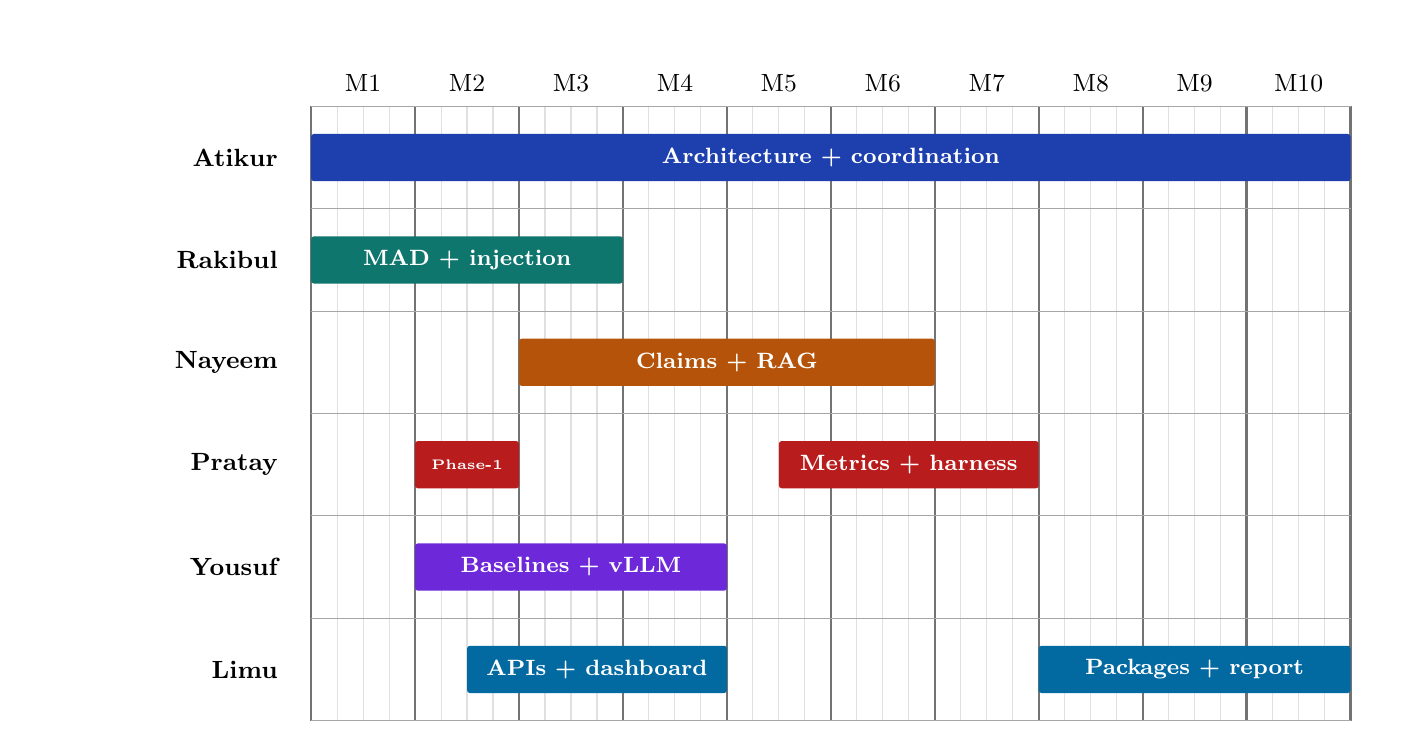
\begin{tikzpicture}[
        wkline/.style={draw=black!12},
        monline/.style={draw=black!55, thick},
        bar/.style={rounded corners=1pt, text=white, font=\footnotesize\bfseries},
        mlab/.style={font=\small},
        nlab/.style={anchor=east, font=\small\bfseries},
      ]
      \definecolor{navy}{HTML}{1E40AF}
      \definecolor{tealg}{HTML}{0F766E}
      \definecolor{amberg}{HTML}{B45309}
      \definecolor{roseg}{HTML}{B91C1C}
      \definecolor{purpg}{HTML}{6D28D9}
      \definecolor{skyg}{HTML}{0369A1}
      \def\s{0.33}
      \path[use as bounding box] (-3.6,0) rectangle (13.7,8.8);
      \foreach \w in {0,...,40} {\draw[wkline] (\w*\s,0) -- (\w*\s,7.8);}
      \foreach \m in {0,...,10} {\draw[monline] (\m*4*\s,0) -- (\m*4*\s,7.8);}
      \foreach \m in {1,...,10} {\node[mlab] at ({(2*\m-1)*2*\s},8.1) {M\m};}
      \foreach \y in {0,...,6} {\draw[black!35] (0,\y*1.3) -- (40*\s,\y*1.3);}
      \node[nlab] at (-0.3,7.15) {Atikur};
      \node[nlab] at (-0.3,5.85) {Rakibul};
      \node[nlab] at (-0.3,4.55) {Nayeem};
      \node[nlab] at (-0.3,3.25) {Pratay};
      \node[nlab] at (-0.3,1.95) {Yousuf};
      \node[nlab] at (-0.3,0.65) {Limu};
      \fill[bar, fill=navy] (0,6.85) rectangle (40*\s,7.45) node[midway] {Architecture + coordination};
      \fill[bar, fill=tealg] (0,5.55) rectangle (12*\s,6.15) node[midway] {MAD + injection};
      \fill[bar, fill=amberg] (8*\s,4.25) rectangle (24*\s,4.85) node[midway] {Claims + RAG};
      \fill[bar, fill=roseg] (4*\s,2.95) rectangle (8*\s,3.55) node[midway, font=\tiny\bfseries] {Phase-1};
      \fill[bar, fill=roseg] (18*\s,2.95) rectangle (28*\s,3.55) node[midway] {Metrics + harness};
      \fill[bar, fill=purpg] (4*\s,1.65) rectangle (16*\s,2.25) node[midway] {Baselines + vLLM};
      \fill[bar, fill=skyg] (6*\s,0.35) rectangle (16*\s,0.95) node[midway] {APIs + dashboard};
      \fill[bar, fill=skyg] (28*\s,0.35) rectangle (40*\s,0.95) node[midway] {Packages + report};
    \end{tikzpicture}}
  \caption{Gantt view of member activity across the ten project months, following the phase plan in Table~\ref{tab:phases}.}
  \label{fig:task-gantt}
\end{figure}

Each task has an identified owner and a simple deliverable. As the owner matches the phase in Table~\ref{tab:phases};all phases will have at least one accountable team member. All dependencies are ordered. Vanilla reproduction will be completed before Injection begins; the Injection Harness completes before Trust Build begins. Dry Run must be passed before Main Experiments begin; Human Evaluation waits for Results Freeze. Writing utilizes the frozen results and occurs last. Each Module is reviewed by the Leader prior to being marked complete. A weekly Git commit and brief stand-up meeting monitor slippage; if any gates are missed, a "fix" week will occur prior to beginning the next phase.

\section{Summary}

Chapter 3 fixed the functional and nonfunctional requirements and drew the
system boundary in the context diagram. The data flow diagram and the interface
design follow. The design section compared the main alternatives and recorded
why each choice was made. The project plan then locks eight phases and six
gates that carry the work to the final defence. Implementation and evaluation
come next.
